\documentclass[a4paper]{article}
\setcounter{secnumdepth}{0}
\usepackage{graphicx}
\usepackage{listings}
\usepackage{amsmath}
\usepackage{cite}
\usepackage{times}
\usepackage{float}

\begin{document}


\title{ELEC5507 Assignment}
\author{Vanush Vaswani - 308196465 \\
Zhaoyan Liu - 440092733 \\
Stephen Tridgell - 309205867}

\maketitle
\newpage
\tableofcontents
\listoffigures
\listoftables


\lstset{language=Matlab, frame=single, breaklines=true, keepspaces=true, columns=flexible, basicstyle=\ttfamily\footnotesize}
\newpage

\part*{Project Introduction}
% i don't think we need this
%\addcontentsline{toc}{part}{Project Introduction}

The goal of error control coding is to encode messages for transmission with redundancy such that the receiver can correct the errors in the transmission and recover the original data. In this project, encoders and decoders will be simulated and analysed by using MATLAB. The first section involves the design and simulation of the BCH code over BSC and AWGN channels. The second section uses LDPC codes to meet the requirements of a power limited system with very high reliability. Similar simulations are run and compared with the results of the BCH code.

\part*{Section I - BCH code}
\addcontentsline{toc}{part}{Section I - BCH code}

\subsubsection{Question 1} \textit{What is the generator polynomial for this code? Use MATLAB’s ’bchgenpoly’ function to verify your answer} \\
\\
The generator polynomial for a n = 31, k = 16, and t = 3 BCH code is $g(x) = x^{15} + x^{11} + 
x^{10} + x^{9} + x^{8} + x^{7} + x^{5} + x^{3} + x^{2} + x^{1} + 1$. 
This was verified with 
\begin{lstlisting}
[gen, t] = bchgenpoly(31,16)
\end{lstlisting}

\subsubsection{Question 2} \textit{What is the minimum distance of this code?} \\
\\
For a BCH code, $d_{min} \geq 2*t + 1 = 7$, this was verified using 
\begin{lstlisting}
gfweight(double(gen.x), 31)
\end{lstlisting}
which gave a minimum distance calculation of 7.

\subsubsection{Question 3} \textit{Construct the reduced syndrome lookup table for this code. You need to write a program to do this since it is difficult to do it by hand. You do not need to include the whole array in your report due to its large size. Instead, just show the sub-array consisting of the first 5 rows in your report, and include a separate text file (*.txt) enumerating all the data in your electronic submission.} \\
\\
Generate the full syndrome lookup table by:
\begin{lstlisting}
[h g k] = cyclgen(31, double(gen.x))
trt = syndtable(h)
\end{lstlisting}
This table can be reduced in size for more efficient implementation by using the cyclic properties of the BCH code. It is calculated in the script \textit{computeReduced.m}. The first 5 rows are:\\
\scalebox{0.7}{
\begin{tabular}{| *{31}{c} |}
\hline
0 & 0 & 0 & 0 & 0 & 0 & 0 & 0 & 0 & 0 & 0 & 0 & 0 & 0 & 0 & 0 & 0 & 0 & 0 & 0 & 0 & 0 & 0 & 0 & 0 & 0 & 0 & 0 & 0 & 0 & 0 \\
\hline
0 & 0 & 0 & 0 & 0 & 0 & 0 & 0 & 0 & 0 & 0 & 0 & 0 & 0 & 0 & 0 & 0 & 0 & 0 & 1 & 0 & 0 & 0 & 0 & 0 & 0 & 1 & 0 & 1 & 0 & 0 \\
\hline
0 & 0 & 0 & 0 & 0 & 0 & 0 & 0 & 0 & 0 & 0 & 0 & 0 & 0 & 0 & 0 & 0 & 0 & 1 & 0 & 1 & 0 & 0 & 0 & 0 & 0 & 0 & 0 & 1 & 0 & 0 \\
\hline
0 & 0 & 0 & 0 & 0 & 0 & 0 & 0 & 0 & 0 & 0 & 0 & 0 & 0 & 0 & 0 & 0 & 1 & 0 & 0 & 0 & 0 & 0 & 0 & 0 & 0 & 0 & 0 & 1 & 0 & 1 \\
\hline
0 & 0 & 0 & 0 & 0 & 0 & 0 & 0 & 0 & 0 & 0 & 0 & 0 & 0 & 0 & 0 & 0 & 1 & 0 & 0 & 0 & 0 & 0 & 1 & 0 & 0 & 0 & 0 & 1 & 0 & 0 \\
\hline
\end{tabular}
}
The corresponding syndromes for these error patterns are:\\
\begin{tabular}{| *{15}{c} | c c |}
\hline
0 & 0 & 0 & 0 & 0 & 0 & 0 & 0 & 0 & 0 & 0 & 0 & 0 & 0 & 0 & = & 0 \\ 
0 & 0 & 0 & 0 & 0 & 0 & 0 & 1 & 0 & 1 & 1 & 0 & 0 & 1 & 1 & = & 179\\
0 & 0 & 0 & 0 & 0 & 1 & 0 & 0 & 0 & 0 & 1 & 1 & 0 & 1 & 1 & = & 539\\
0 & 0 & 0 & 0 & 0 & 1 & 1 & 0 & 0 & 0 & 0 & 1 & 1 & 0 & 1 & = & 781\\
0 & 0 & 0 & 1 & 0 & 0 & 0 & 0 & 0 & 0 & 1 & 0 & 1 & 1 & 1 & = & 2071\\
\hline
\end{tabular}\\
\\
The rest of the array is in \textit{reducedSyndromeTable.csv}. This contains the error pattern in binary then the decimal representation of the syndrome with the left bit as the most significant bit.

\subsubsection{Question 4} \textit{Based on the standard array you obtained in task 3, find out the weight distribution of the coset leaders.}\\
\\
For the full syndrome table, or standard array coset leaders, the weight distribution is calculated as follows:
\begin{lstlisting}
weights = sum(trt')
A0 = sum(weights == 0)
A1 = sum(weights == 1)
A2 = sum(weights == 2)
A3 = sum(weights == 3)
A4 = sum(weights == 4)
A5 = sum(weights == 5)
\end{lstlisting}
Gives the weight distribution of $A_0 = 1$, $A_1 = 31$, $A_2 = 465$, $A_3 = 4495$, $A_4 = 13020$ and $A_5 = 14756$ where $A_i$ is the number of weight $i$ errors. This is the number of possible combinations up to $A_3$ where $A_i$ = $ 31 \choose i$. Similarly the weight distribution of the reduced syndrome table is calculated. This gave the weight distribution of $A_0 = 1$, $A_1 = 1$, $A_2 = 15$, $A_3 = 145$, $A_4 = 840$ and $A_5 = 2835$. This can be verified for $A_1$, $A_2$ and $A_3$ as they contain 31 cycles of all words. Hence the total for $A_3$ is $ \frac{{31 \choose 3}}{31} = 145$.

\subsubsection{Question 5} \textit{Design and implement an encoder using the generator polynomial for this BCH code.} \\
\\
The encoder with the generator polynomial was implemented using the cyclic properties of the code. The message, $c(X)$, is shifted by $n-k$ and divided by the generator polynomial to get the parity check bits by $b(X) = remainder[\frac{X^{n-k}c(X)}{g(X)}]$. The parity check bits are combined with the message for a systematic code. The function \textit{polBCHencoder.m} implements the generator polynomial method of decoding the BCH code.

\subsubsection{Question 6a} \textit{Use MATLAB defined functions (eg. the ”decode” function) to decode the BCH code.}\\
\\
This decoder is implemented using MATLAB’s function \textit{decode()}. The matrix \textit{trt} is the syndrome decoding table calculated above using the \textit{syndtable()} function. This decode method is based on the block properties of the code. The syndromes are calculated and the most likely codeword is decoded to by looking up the minimum weight. Th implementation is in the function \textit{matlabBCHdecode.m}.

\subsubsection{Question 6b} \textit{Design and implement a decoder using the syndrome decoding table in Task 3 for the BCH code.}\\
\\
The syndrome can be obtained by multiplying received codeword with the transposed parity-check matrix H. The corresponded error pattern is found by performing a look up in the trt table calculated above. The corrected code is then the codeword plus the error pattern. Our implementation is shown in the function \textit{syndLookupDecode.m}. The overhead of the decoder can be reduced by significantly reducing the size of the lookup table by using cyclic properties of the code. This was implemented using the reduced lookup table calculated previously. The recieved vector is shifted until its syndrome is recognized in the table. The error locations are then looked up in the table. The implementation of this is in \textit{syndReducedLookupDecode.m}

\subsubsection{Question 6c} \textit{Design and implement a decoder using the Berlekamp’s iterative procedure.}\\
\\
The implementation of Berlekamp's iterative procedure below used different notation to the textbook specified in \textit{http://www.mathworks.com.au/help/comm/ug/error-detection-and-correction.html} allowing easier implementation of the procedure. See the function \textit{berlekamp\_decode.m} for the matlab code. 

\begin{figure}[H]
\centering
\includegraphics[scale=0.4]{berlekamp.png}
\caption{Flow chart of berlekamps from www.mathworks.com.au/help/comm/ug/error-detection-and-correction.html}
\end{figure}

This differs from the textbook method in its labeling of variables, but additionally a slight modification on the calculation of $\sigma_{\rho}$. It instead computes the this as the variable D with $d_{\rho}$ alread divided through. This allows for easier implementation in software.

\subsection{Sound analysis}

\subsubsection{Question 7} \textit{Simulate the implemented BCH encoder and decoder (using ANY method in Part 6) using the attached wave file (austinpowers.wav) in a BSC channel for different transition probabilities. Discuss the impact of changing different transition probability values.}\\
\\
The channel was simulated using the function \textit{playAudioOverBSC.m}. Different transition probabilities were input into the function. With a transition probability of below 0.05 the sound could be heard with a little noise audible. As p increased above 0.15 the noise increased to the level where it could no longer be clearly heard. Above 0.2 it was difficult to hear anything at all other than noise.

The plots for different p-values are shown below as a qualitative indicator of noise levels.

\begin{figure}[H]
\centering
\includegraphics[scale=0.5]{plots/audio_over_bsc_bch_p_001.png}
\caption{BCH Audio over BSC (p = 0.01)}
\end{figure}

\begin{figure}[H]
\centering
\includegraphics[scale=0.5]{plots/audio_over_bsc_bch_p_005.png}
\caption{BCH Audio over BSC (p = 0.05)}
\end{figure}

\begin{figure}[H]
\centering
\includegraphics[scale=0.5]{plots/audio_over_bsc_bch_p_010.png}
\caption{BCH Audio over BSC (p = 0.1)}
\end{figure}

\subsection{BER analysis}

\subsubsection{Question 8a and 8b} \textit{Simulation over BSC Simulate the BCH code in a BSC channel (you are allowed to use MATLAB defined functions) and plot the BER versus transition probability for coded and uncoded systems on the same graph. Plot BER versus $\frac{E_b}{N_0}$ for coded and uncoded systems on the same graph by assuming that the SNR ($ = \frac{E_b}{N_0}$ ) is related to the transition probability for the coded system via $X_{dB,coded} = 10 \log_{10}(\frac{[Q^{- 1} (p)]^2}{R}) $ and that for uncoded system is $X_{dB,uncoded} = 20\log_{10}(Q^{- 1} (p)) $, where $Q(x) = \frac{1}{\sqrt{2 \pi}} \int\limits_{x}\limits^{+\infty} e^{ -\frac{z^2}{2}} dz $ and $0 < p < 0.5$.}\\
\textit{Simulation over AWGN channel with BPSK modulation $\{-1, 1\}$ Simulate the BCH code in an AWGN channel (you are allowed to use MATLAB defined functions) and plot the BER versus the signal to noise ratio (SNR) for a BPSK coded and uncoded systems on the same graph by using a hard-decision demodulator and binary decoder.}\\
\\
The implementation of the simulation is in \textit{bch\_ber\_simulation.m}.
This produced the following plots. \\
\begin{figure}[H]
\centering
\includegraphics[scale=0.5]{plotBER_BSC_pvals.jpg} \\
\caption{Bit Error Rate vs. transition probability for BCH over BSC}
\end{figure}

\begin{figure}[H]
\centering
\includegraphics[scale=0.5]{plotBER_BSC_SNR.jpg}
\caption{Bit Error Rate vs. SNR for BCH over BSC}
\end{figure}

\begin{figure}[H]
\centering
\includegraphics[scale=0.5]{plotBER_AWGN.jpg} 
\caption{Bit Error Rate vs. SNR for BCH over AWGN}
\end{figure}
\textbf{TODO: RESAVE AWGN plot} 

\subsubsection{Question 8c} \textit{Draw a table detailing the coding gain for BER$= [10^{-2}, 10^{-3}, 10^{-4} , 10^{-5} , 10^{-6} ]$ by reading the differences between the BER curves for BPSK coded and uncoded systems which have been obtained from simulations in part (a) and (b).} \\
\\
\begin{table}[H]
\centering
\begin{tabular}{| c | c | c |}
\hline
BER & Coding Gain (Hard decision) & Coding Gain (BSC) \\
\hline
$10^{-2}$ & & \\
\hline
$10^{-3}$ & & \\
\hline
$10^{-4}$ & & \\
\hline
$10^{-5}$ & & \\
\hline
$10^{-6}$ & & \\
\hline

\end{tabular}
\caption{Coding gain for BCH}
\end{table}

\subsubsection{Question 8d} \textit{Find the asymptotic coding gain when $\frac{Eb}{N0}$ is very large from the formula which is given in the lecture notes and compare with simulation results.} \\
\\
Using the formula $G = 10\log(R(t+1))$ in lecture 5 for large $\frac{Eb}{N0}$ where $R = 16/31$ and $t = 3$ results in a coding gain of $G = 3.1482$ dB. Comparing this to the simulation results \textbf{... TODO!!!} \\

% =========
% SECTION 2
% =========

\hrulefill
\newpage

\part*{Section II - LDPC}
%\addcontentsline{toc}{part}{Section II - LDPC}


\textit{You are an engineer whose job is to design and analyze the performance of error control codes for different clients. Client 2 requires a code for satellite transmission of digital TV. The satellite is power limited and very high reliability is required (as close to Shannon capacity as possible). Low decoding complexity is desired, but is not essential.} 

\subsubsection{Question 1} \textit{Design the code (e.g. type of code, code parameters, and other relevant information) and justify its design}

%% ANSWER 
%% ======
To meet these requirements an LDPC code is used

For client 2, it is clear that an LDPC code will be necessary and these can provide performance that is close to the Shannon limit for an AWGN channel, compared to other modern codes. However, it is known that this is the case for very long block codes, which require computationally complex [TODOREF].
An existing solution for digital satellite television is present in the DVB-S2
standard, which uses LDPC as part of concatenated code with BCH coding\cite{morello2006dvb}. However,
the drawback of this scheme is the high decoding complexity, though this can be 
reduced somewhat by the special structure of the code [TODOREF]. Another factor to consider is the power limitation of the satellite, since a large LDPC block code will also entail high coding complexity, more hardware gates and thus more power. An alternative code choice
is the (1152, 2304) LDPC block code used in IEEE-802.16-2005, also known as WiMax [TODOREF]. This code is also irregular, which is known to exhibit superior performance over regular LDPC codes.

TODO: Expand on justification, summarize into table

\subsection{Sound analysis}

\subsubsection{Question 2} \textit{Simulate the chosen code using the attached wave file (austinpowers.wav) in a BSC channel for different transition probabilities (you are allowed to use MATLAB defined functions. Discuss the difference in sound quality compared to the BCH code in Section I, for different transition probabilities.}\\
\\

%% ANSWER 
%% ======

The code was simulated for the transition probabilities p = \{0.01, 0.05, 0.1\}. As a qualitative tool, plots of the waveform are included. Figures 1-3 provide a visual indicator of the noise. \\

\begin{figure}[H]
\centering
\includegraphics[scale=0.5]{plots/audio_over_bsc_ldpc_p_001.png}
\caption{LDPC Audio over BSC (p = 0.01)}
\end{figure}

\begin{figure}[H]
\centering
\includegraphics[scale=0.5]{plots/audio_over_bsc_ldpc_p_005.png}
\caption{LDPC Audio over BSC (p = 0.05)}
\end{figure}

\begin{figure}[H]
\centering
\includegraphics[scale=0.5]{plots/audio_over_bsc_ldpc_p_010.png}
\caption{LDPC Audio over BSC (p = 0.1)}
\end{figure}

As the bit errors increase due to the transition probability, the noise becomes more prevalent. However, it is improved relative to BCH in the case of p = 0.05, showing LDPC has superior performance in this regard compared with BCH. However, there is not much difference in the case of p = 0.1, showing that the code has reached it's performance limitation for the particular channel, which is due to effective hard-decision decoding that is involved in a BSC channel. TODO: is it?

\subsubsection{Question 3a}\textit{Simulate the chosen code in a BSC channel (you are allowed to use MATLAB defined functions) and plot the BER versus transition probability for coded and uncoded systems on the same graph. Plot BER versus $\frac{E_b}{N_0}$ for coded and uncoded systems on the same graph by assuming that the SNR ($ = \frac{E_b}{N_0}$ ) is related to the transition probability for the coded system via $X_{dB,coded} = 10 \log_{10}(\frac{[Q^{-1} (p)]^2}{R}) $ and that for uncoded system is $X_{dB,uncoded} = 20\log_{10}(Q^{-1} (p)) $, where $Q(x) = \frac{1}{\sqrt{2 \pi}} \int\limits_{x}\limits^{+\infty} e^{ -\frac{z^2}{2}} dz $ and $0 < p < 0.5$.}

\begin{figure}[H]
\centering
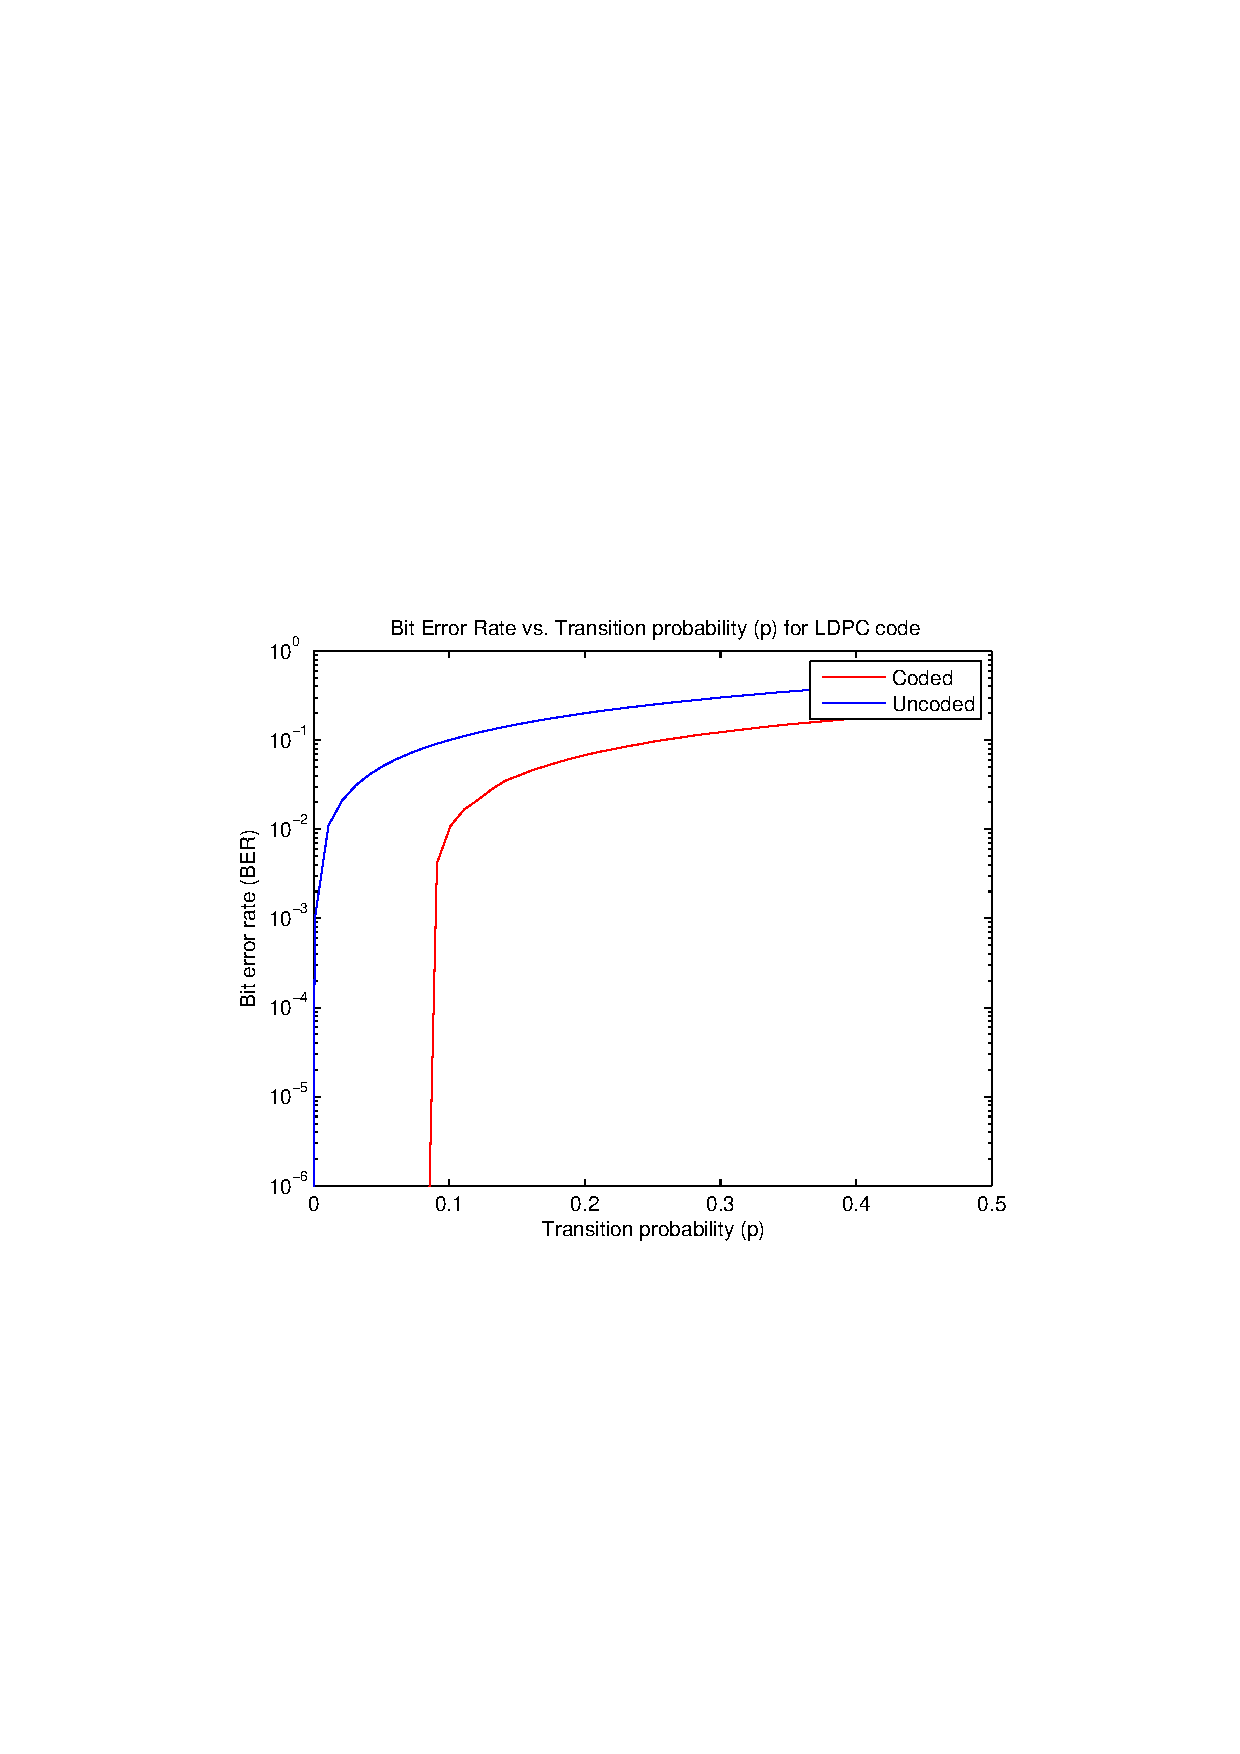
\includegraphics[scale=0.5]{plots/ber_vs_p_ldpc.png}
\caption{BER vs transition probability for LDPC over BSC}
\end{figure}

\begin{figure}[H]
\centering
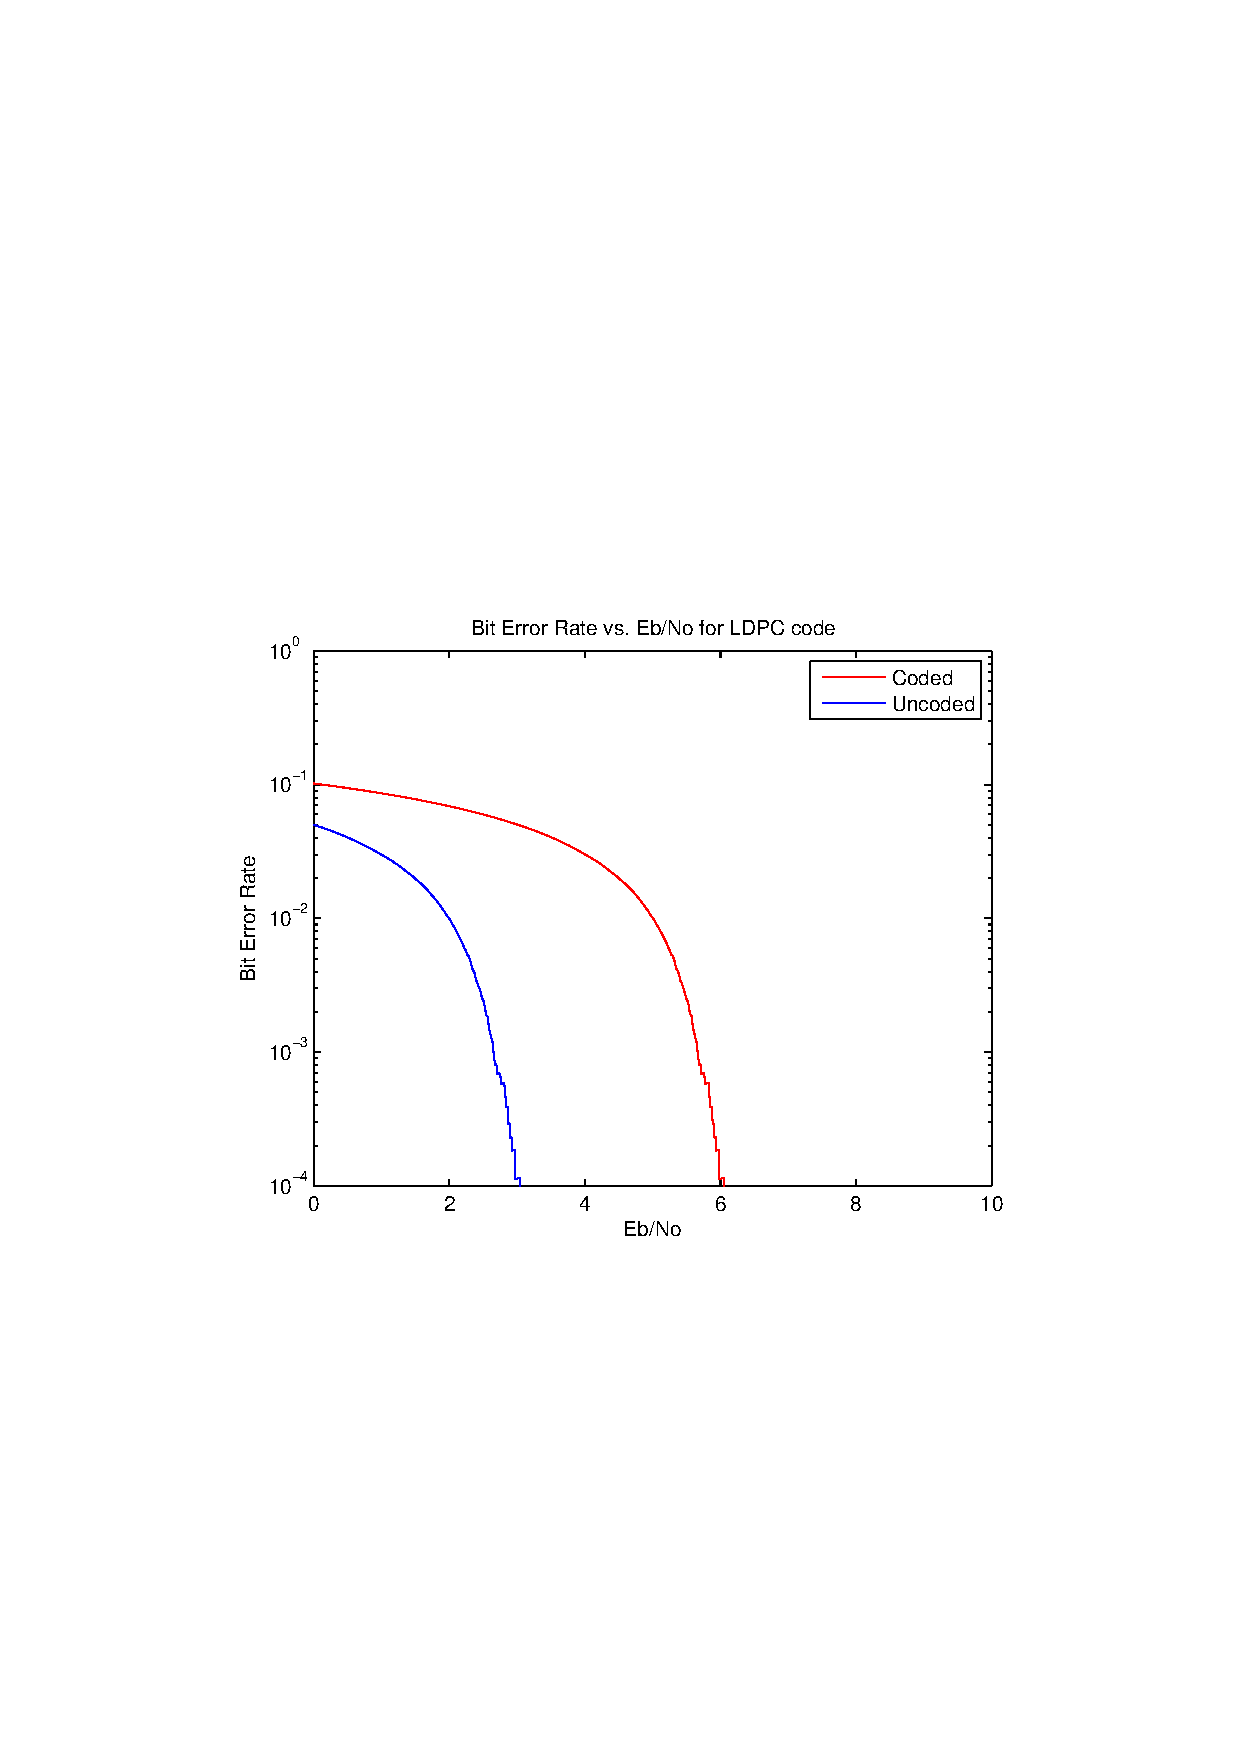
\includegraphics[scale=0.5]{plots/ber_vs_ebno_ldpc.png}
\caption{BER vs EbNo for LDPC over BSC}
\end{figure}


\subsection{BER analysis}

\subsubsection{Question 3b} \textit{Simulate the chosen code in an AWGN channel (you are allowed to use MATLAB defined functions) and plot the BER versus the signal to noise ratio (SNR) for a BPSK coded and uncoded systems on the same graph by using a hard-decision demodulator and binary decoder. Simulate the chosen code in an AWGN channel and plot the BER versus SNR on the same graph for a BPSK coded system by using a soft-decision decoder.}

\begin{figure}[H]
\centering
\includegraphics[scale=0.5]{plots/ber_vs_ebno_ldpc_awgn_hard.png}
\caption{BER vs EbNo for Hard-decision demod and decoding (LDPC - AWGN)}
\end{figure}

\begin{figure}[H]
\centering
\includegraphics[scale=0.5]{plots/ber_vs_ebno_ldpc_awgn_soft.png}
\caption{BER vs EbNo for Soft-decision demod and decoding (LDPC - AWGN)}
\end{figure}


\subsubsection{Question 3c} \textit{Draw a table detailing the coding gain for BER$= [10^{-2}, 10^{-3}, 10^{-4} , 10^{-5} , 10^{-6} ]$ by reading the differences between the BER curves for BPSK coded and uncoded systems which have been obtained from simulations in part (a) and (b).}\\
\\

\begin{table}[H]
\centering
\begin{tabular}{| c | c | c | c |}
\hline
BER &  Coding Gain (Hard decision) & Coding Gain (Soft decision)  & Coding Gain (BSC\\
\hline
$10^{-2}$ & & & \\
\hline
$10^{-3}$ & & & \\
\hline
$10^{-4}$ & & & \\
\hline
$10^{-5}$ & & & \\
\hline
$10^{-6}$ & & & \\
\hline
\end{tabular}
\caption{Coding gain for LDPC}
\end{table}

\subsubsection{Question 3d} \textit{Find the asymptotic coding gain when $\frac{Eb}{N0}$ is very large from the formula which is given in the lecture notes and compare with simulation results.} \\
\\
Answer here \\

\subsubsection{Question 4} \textit{Discuss the advantages/disadvantages of the code chosen in this section with the BCH code in Section 1 (eg. complexity, coding gain, efficiency)}\\
\\
BCH codes have significantly lower complexity than the LDPC as BCH has the properties that it is a cyclic, linear block code. This allows various decoding methods depending on resources availible. BCH can also be systematic allowing for simpler decoding methods. LDPC codes are additionally large in size generally, compared to the BCH codes. This means that there is greater latency in the delivery of data. LDPC however, performs significantly better than BCH in terms of coding gain ... etc

\bibliographystyle{plain}
\bibliography{refs}

\hfill
\newpage

\part*{Appendix - Matlab code}

\lstinputlisting{../bch_ber_simulation.m}
\lstinputlisting{../computeReduced.m} 
\lstinputlisting{../matlabBCHdecode.m} 
\lstinputlisting{../polBCHencoder.m} 
\lstinputlisting{../syndReducedLookupDecode.m}
\lstinputlisting{../berlekamp_decode.m} 
\lstinputlisting{../encoder.m} 
\lstinputlisting{../playAudioOverBSC.m} 
\lstinputlisting{../syndLookupDecode.m}
\lstinputlisting{../ldpc/binary_to_wav.m}
\lstinputlisting{../ldpc/plot_ebno.m  } 
\lstinputlisting{../ldpc/simulate_ldpc_awgn_hard.m  } \lstinputlisting{../ldpc/simulate_ldpc_bsc.m  } 
\lstinputlisting{../ldpc/wav_to_binary.m}
\lstinputlisting{../ldpc/plot_ber.m } 
\lstinputlisting{../ldpc/qpsk_test.m  } 
\lstinputlisting{../ldpc/simulate_ldpc_awgn_soft.m  } \lstinputlisting{../ldpc/simulate_ldpc_wav.m}

\end{document}